\documentclass[aspectratio=169]{beamer}
%%%%%%%%%%%%%%%%%%%%%%%%%%%%%%%%%%%%%%%%%
% Beamer Presentation
% LaTeX Template
% Version 1.0 (10/11/12)
%
% This template has been downloaded from:
% http://www.LaTeXTemplates.com
%
% License:
% CC BY-NC-SA 3.0 (http://creativecommons.org/licenses/by-nc-sa/3.0/)
%
%%%%%%%%%%%%%%%%%%%%%%%%%%%%%%%%%%%%%%%%%

%----------------------------------------------------------------------------------------
%	PACKAGES AND THEMES
%----------------------------------------------------------------------------------------

\usepackage[portuges]{babel}
\usepackage[utf8]{inputenc}
\usepackage[alf]{abntex2cite}	
\usepackage[portuguese, linesnumbered, vlined, titlenumbered, ruled]{algorithm2e}
\SetKwRepeat{Registro}{registro \{}{\}}%
\usepackage{beamerthemesplit}
\usepackage{multirow}
\usepackage{scalefnt}

% The Beamer class comes with a number of default slide themes
% which change the colors and layouts of slides. Below this is a list
% of all the themes, uncomment each in turn to see what they look like.

%\usetheme{default}
%\usetheme{AnnArbor}
%\usetheme{Antibes}
%\usetheme{Bergen}
%\usetheme{Berkeley}
%\usetheme{Berlin}
%\usetheme{Boadilla}
%\usetheme{CambridgeUS}
%\usetheme{Copenhagen}
%\usetheme{Darmstadt}
%\usetheme{Dresden}
%\usetheme{Frankfurt}
%\usetheme{Goettingen}
%\usetheme{Hannover}
%\usetheme{Ilmenau}
%\usetheme{JuanLesPins}
%\usetheme{Luebeck}
\usetheme{Madrid}
%\usetheme{Malmoe}
%\usetheme{Marburg}
%\usetheme{Montpellier}
%\usetheme{PaloAlto}
%\usetheme{Pittsburgh}
%\usetheme{Rochester}
%\usetheme{Singapore}
%\usetheme{Szeged}
%\usetheme{Warsaw}

% As well as themes, the Beamer class has a number of color themes
% for any slide theme. Uncomment each of these in turn to see how it
% changes the colors of your current slide theme.

%\usecolortheme{albatross}
%\usecolortheme{beaver}
%\usecolortheme{beetle}
%\usecolortheme{crane}
\usecolortheme{dolphin}
%\usecolortheme{dove}
%\usecolortheme{fly}
%\usecolortheme{lily}
%\usecolortheme{orchid}
%\usecolortheme{rose}
%\usecolortheme{seagull}
%\usecolortheme{seahorse}
%\usecolortheme{whale}
%\usecolortheme{wolverine}

%\setbeamertemplate{footline} % To remove the footer line in all slides uncomment this line
%\setbeamertemplate{footline}[page number] % To replace the footer line in all slides with a simple slide count uncomment this line

%\setbeamertemplate{navigation symbols}{} % To remove the navigation symbols from the bottom of all slides uncomment this line


\usepackage{graphicx} % Allows including images
\usepackage{booktabs} % Allows the use of \toprule, \midrule and \bottomrule in tables

%----------------------------------------------------------------------------------------
%	TITLE PAGE
%----------------------------------------------------------------------------------------

\title[Árvores Binárias de Busca]{Algoritmos e Estrutura de Dados}
\subtitle{Árvores Binárias de Busca}
\author[Frederico Santos de Oliveira]{prof. Frederico Santos de Oliveira}
\institute[UFMT]{Universidade Federal de Mato Grosso\\ Faculdade de Engenharia}
\date{}

\begin{document}

%------------------------------------------------
\begin{frame}
\titlepage % Print the title page as the first slide

\begin{figure}[!h]
  \centering
   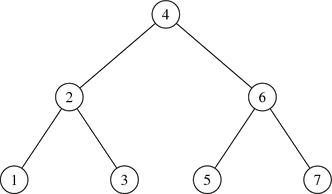
\includegraphics[width=120pt]{imagens/introducao.png}
  \label{fig_introducao}
\end{figure}
\end{frame}

%------------------------------------------------

\begin{frame}
\frametitle{Roteiro} % Table of contents slide, comment this block out to remove it
\tableofcontents % Throughout your presentation, if you choose to use \section{} and \subsection{} commands, these will automatically be printed on this slide as an overview of your presentation
\end{frame}

%----------------------------------------------------------------------------------------
%	PRESENTATION SLIDES
%----------------------------------------------------------------------------------------

%------------------------------------------------
\section{Objetivos}

\begin{frame}
\frametitle{Objetivos}

Esta aula tem como objetivos:

\begin{enumerate}
\item Apresentar os conceitos básicos sobre árvores binárias de busca (ABBs);
\item Exemplificar os algoritmos de manipulação de ABBs por meio de pseudo-códigos.
\end{enumerate}

\end{frame}

%------------------------------------------------
% 
% \section{Referências bibliográficas}
%   \frame{\frametitle{Referências bibliográficas}
%     \bibliographystyle{abntex2-alf}
%     \bibliography{referencias}
%   }
%   
%------------------------------------------------
\section{Introdução} % Sections can be created in order to organize your presentation into discrete blocks, all sections and subsections are automatically printed in the table of contents as an overview of the talk
%------------------------------------------------


\begin{frame}{Árvore Binária de Busca}{Introdução}
\begin{itemize}
 \item Um Árvore Binária de Busca (ABB) é um tipo especial de árvore binária, ou seja, possui as mesmas propriedades de uma árvore binária.
 \item No entanto, na ABB o  item armazenado no nodo determina a sua posição na árvore.
 \item Em uma ABB, temos a seguinte regra para posicionamento dos valores na árvore, para cada nodo {\bf pai}:
 \begin{itemize}
 \item Todos os valores da subárvore {\bf esquerda} são {\bf menores} do que o nodo pai.
 \item Todos os valores da subárvore {\bf direita} são {\bf maiores} do que o nodo pai.
 \end{itemize} 
\end{itemize}
\end{frame}

% -----------------------------------

\begin{frame}{Árvore Binária de Busca}{Exemplo}

\begin{figure}[!h]
  \centering
  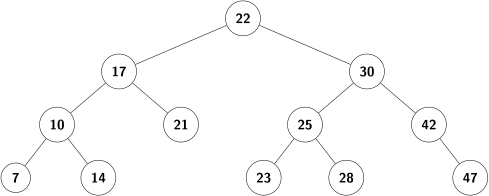
\includegraphics[width=250pt]{imagens/abb.png}
  \label{fig_abb}
\end{figure}
\end{frame}

\section{Implementação}


\begin{frame}{Árvore Binária de Busca}{Operações}
A seguir, são apresentados os seguintes algoritmos sobre ABBs:
\begin{enumerate}
 \item Busca
 \item Inserção
 \item Remoção
\end{enumerate}
\end{frame}



\subsection{Busca}


%------------------------------------------------

\begin{frame}{Árvore Binária de Busca}{Busca}
A seguir, são apresentados duas versões do algoritmo de busca:
\begin{enumerate}
 \item Uma versão {\bf recursiva}
 \item Uma versão {\bf iterativa}
\end{enumerate}
\end{frame}

%------------------------------------------------

\begin{frame}{Árvore Binária de Busca}{Busca Recursiva}
\begin{itemize}
 \item Algoritmos recursivos possuem pelo menos um {\bf caso base} e um {\bf caso recursivo}.
 \item O caso base resolve o problema, ou seja, encontra ou não o elemento na árvore:
 \begin{itemize}
 \item Retorna NULL quando o elemento não foi encontrado.
 \item Retorna um ponteiro para o elemento procurado, caso tenha sido encontrado.
 \end{itemize}
 \item Existem dois casos recursivos:
 \begin{itemize}
 \item O primeiro ocorre quando o elemento procurado é \underline{menor} que o valor armazenado no nodo raiz .
 \begin{itemize}
 \item Nesse caso, busca-se {\bf recursivamente} na subárvore da \underline{esquerda}.
 \end{itemize}
 \item O segundo caso ocorre quando o valor procurado é \underline{maior} que o valor armazenado no nodo raiz.
 \begin{itemize}
 \item Nesse caso, busca-se {\bf recursivamente} na subárvore da \underline{direita}.
 \end{itemize} 
 \end{itemize}
\end{itemize}
\end{frame}

%------------------------------------------------

\begin{frame}{Árvore Binária de Busca}{Função Buscar - Versão Recursiva}
% \scalebox{0.8}{
\begin{algorithm}[H]
\caption{Busca} 
\label{BuscarRecursivo}
\Entrada{Ponteiro para a raiz $r$ e o item $x$ a ser procurado.}
\Saida{Retorna o nodo que contém o item $x$ ou NULL caso não encontrado.}
\Inicio{
    \Se {(r = NULL) ou (x = r.item)} {
      \Retorna r
    }
    \SenaoSe{(x $>$ r.item)} {
	  \Retorna Buscar(r.dir)
    } 
    \Senao {
	  \Retorna Buscar(r.esq)
    }
}
\end{algorithm}
% }  
\end{frame}



%------------------------------------------------

\begin{frame}{Árvore Binária de Busca}{Busca Iterativa}
\begin{itemize}
 \item O algoritmo iterativo utiliza um laço de repetição ({\bf enquanto}) para caminhar na árvore.
 \item Para isso, utiliza um ponteiro auxiliar, chamado {\bf atual}:
\begin{itemize}
\item Percorre a árvore a fim de encontrar o elemento procurado.
\end{itemize}
\item O laço termina em duas situações:
\begin{itemize}
\item Quando {\bf (atual = NULL)}, o que indica que o elemento não foi encontrado.
\item Ou quando {\bf (atual.item = $x$)}, ou seja, encontrou o elemento procurado.
\end{itemize}
\item Por fim, retorn NULL ou o ponteiro para o elemento encontrado.
\end{itemize}
\end{frame}

\begin{frame}{Árvore Binária de Busca}{Função Buscar - Versão Iterativa}
\scalebox{0.8}{
\begin{algorithm}[H]
\caption{Busca} 
\label{Buscar}
\Entrada{Ponteiro para a raiz $r$ e o item $x$ a ser procurado.}
\Saida{Retorna o nodo que contém o item $x$ ou NULL caso não encontrado.}
\Inicio{indica
    \Se {(r = NULL)} {
      \Retorna NULL
    }
    \Senao {
    	atual $\leftarrow$ r \\
    	\Enqto {(atual $\neq$ NULL) AND (atual.item $\neq x$)} {
			\Se{(x $>$ atual.item)} {
	  			atual $\leftarrow$ atual.dir \\
			}
			\Senao {
	  			atual $\leftarrow$ atual.esq \\
			}
    	}
    	\Retorna atual
    }
}
\end{algorithm}
}  

\tiny{Adaptado de \cite{Backes2016}}
\end{frame}


\begin{frame}{Árvore Binária de Busca}
\begin{itemize}
 \item As operações de inserção e remoção de nodos na ABB devem ser realizadas respeitando as regras de posicionamento dos nodos.
 \item No caso médio, as operações de busca, inserção e remoção possuem tempo de execução $O(\log(n))$ em que $n$ é a quantidade de nodos na árvore.
 \item No entanto, em seu pior caso, as operações de busca, inserção e remoção possuem tempo de execução $O(n)$
\end{itemize}
\end{frame}

\subsection{Inserção}

\begin{frame}{Árvore Binária de Busca}{Inserção}
\begin{itemize}
 \item Inserir um novo nodo em uma ABB é uma tarefa bastante simples.
 \item Basta alocar espaço para o novo nodo e procurar a sua posição na ABB.
 \item A seguir, os passos necessários:
 \begin{enumerate}
  \item Primeiro, compare o valor a ser inserido com a {\bf raiz}.
  \item Se o valor for menor do que a raiz, vá para a subárvore da {\bf esquerda}.
  \item Caso contrário, vá para a subárvore da {\bf direita}.
  \item Aplique o método recursivamente até chegar a um {\bf nodo folha}.
 \end{enumerate}
\end{itemize}
\end{frame}

% -----------------------------------

\begin{frame}{Árvore Binária de Busca}{Inserção}
\begin{figure}[!h]
  \centering
  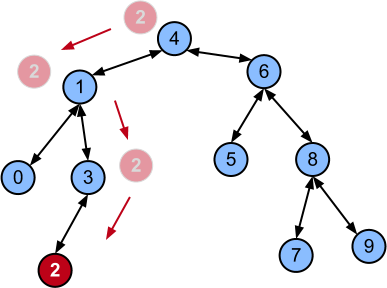
\includegraphics[width=200pt]{imagens/insercao1.png}
  \label{fig_insercao}
\end{figure}
\end{frame}

%------------------------------------------------

\begin{frame}{Árvore Binária de Busca}{Inserção}
A seguir, são apresentados duas versões do algoritmo de inserção:
\begin{enumerate}
 \item Uma versão {\bf recursiva}
 \item Uma versão {\bf iterativa}
\end{enumerate}
\end{frame}


%------------------------------------------------

\begin{frame}{Árvore Binária de Busca}{Inserção Recursiva}
\begin{itemize}
 \item Algoritmos recursivos possuem pelo menos um {\bf caso base} e um {\bf caso recursivo}.
 \item O caso base resolve o problema, ou seja, insere um elemento na árvore:
 \begin{itemize}
 \item Neste algoritmo, o caso base ocorre quando a raiz da árvore (ou subárvore) é igual a NULL.
 \item Nesse caso, cria-se um novo nodo, e este será a raiz da árvore (ou subárvore).
 \end{itemize}
 \item Existem dois casos recursivos:
 \begin{itemize}
 \item O primeiro ocorre quando o elemento a ser inserido é \underline{menor} que o valor armazenado no nodo raiz .
 \begin{itemize}
 \item Nesse caso, insere-se {\bf recursivamente} na subárvore da \underline{esquerda}.
 \end{itemize}
 \item O segundo caso ocorre quando o valor a ser inserido é \underline{maior} que o valor armazenado no nodo raiz.
 \begin{itemize}
 \item Nesse caso, insere-se {\bf recursivamente} na subárvore da \underline{direita}.
 \end{itemize} 
 \end{itemize}
\end{itemize}
\end{frame}


%------------------------------------------------


\begin{frame}{Árvore Binária de Busca}{Inserção - Versão Recursiva}
% \scalebox{0.8}{
\begin{algorithm}[H]
\caption{InserirÁrvore} 
\label{Inserir_arvore_recursivo}
\Entrada{Ponteiro $r$ para raiz, item $x$ a ser inserido na árvore.}
\Inicio{
  \Se{(r=NULL)} {
    novo $\leftarrow$ ALOCA\_NODO() \\
    novo.item $\leftarrow$ x \\
    novo.esq $\leftarrow$ NULL \\
    novo.dir $\leftarrow$ NULL \\               
    r $\leftarrow$ novo \\ 
  }
  \SenaoSe {(x $<$ r.item)} {
      InserirÁrvore(r.esq, x) \\
  } 
  \Senao {
      InserirÁrvore(r.dir, x) \\
  }
}
\end{algorithm}
% }  
\end{frame}

% -----------------------------------

\begin{frame}{Árvore Binária de Busca}{Inserção}
\begin{figure}[!h]
  \centering
  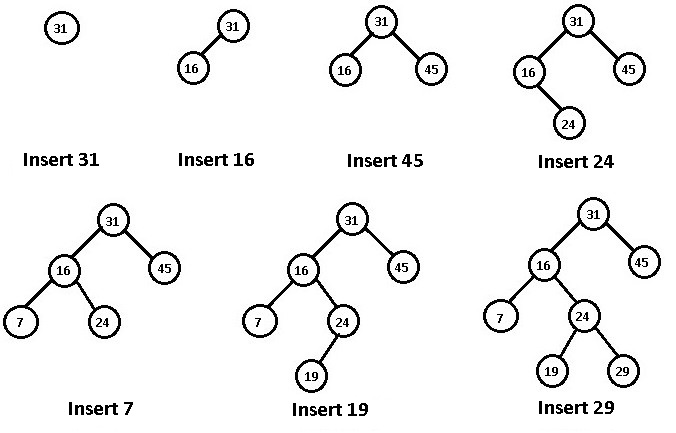
\includegraphics[width=250pt]{imagens/insercao2.jpg}
  \label{fig_insercao2}
\end{figure}
\end{frame}

%------------------------------------------------
\begin{frame}{Árvore Binária de Busca}{Inserção - Versão Iterativa}
\begin{itemize}
\item Na versão iterativa, primeiramente, cria-se o novo nodo que será inserido na árvore.
\item Em seguida, deve-se encontrar a posição em que o novo nodo será inserido na árvore.
\begin{itemize}
\item Para isso, utiliza-se um laço de repetição ({\bf enquanto}) para encontrar a posição em que será inserido o novo elemento.
\item Existem dois ponteiros auxiliares:
\begin{itemize}
\item Atual $\rightarrow$ percorre a árvore a fim de encontrar a posição em que será inserido o novo nodo.
\item Anterior $\rightarrow$ é o nodo anterior ao nodo {\bf atual}, ou seja, o seu pai.
\end{itemize}
\item O laço termina quando {\bf (atual = NULL)}.
\item Por fim, o novo nodo é inserido como filho do nodo {\bf anterior}.
\end{itemize}
\end{itemize}
\end{frame}

%------------------------------------------------

\begin{frame}{Árvore Binária de Busca}{Inserção - Versão Iterativa}
\scalebox{0.55}{
\begin{algorithm}[H]
\caption{InserirÁrvore} 
\label{Inserir_arvore_iterativo	}
\Entrada{Ponteiro $r$ para raiz, item $x$ a ser inserido na árvore.}
\Inicio{
  novo $\leftarrow$ ALOCA\_NODO() \\
  novo.item $\leftarrow$ x \\
  novo.esq $\leftarrow$ NULL \\
  novo.dir $\leftarrow$ NULL \\             
  \Se{(r=NULL)} {
    r $\leftarrow$ novo \\ 
  }
  \Senao {
    atual $\leftarrow$ r \\
    anterior $\leftarrow$ NULL \\
    \Enqto{(atual $\neq$ NULL)} {
      anterior $\leftarrow$ atual \\
      \Se {(novo.item $<$ atual.item)} {
	atual $\leftarrow$ atual.esq \\
      } 
      \Senao {
	atual $\leftarrow$ atual.dir \\
      }
    }
    \Se {(novo.item $<$ anterior.item)} {
      anterior.esq $\leftarrow$ novo \\
    }
    \Senao {
      anterior.dir $\leftarrow$ novo \\
    }
  }
}
\end{algorithm}
}

\tiny{Adaptado de \cite{Backes2016}}  
\end{frame}


\subsection{Remoção}

\begin{frame}{Árvore Binária de Busca}{Remoção}
\begin{itemize}
 \item Para remover um item de uma ABB precisamos procurar o nodo a ser removido, que pode ser um nodo {\bf folha} ou um nó {\bf interno}.
 \begin{itemize}
 \item Caso seja um nodo interno, pode possuir um ou dois filhos.
 \item Um dos filhos substitui o pai e é preciso reorganizar a árvore para que ela continue sendo uma ABB.
 \end{itemize}
 \item Para realizar a remoção de um elemento, será necessário utilizar uma função auxiliar, denominada {\bf RemoverAtual}. 
 \item Essa função auxiliar recebe como parâmetro o endereço de um nodo da árvore ({\bf atual}) a ser removido e retorna qual deverá ser o seu nodo {\bf substituto}, que será o seu antecessor na árvore.
\end{itemize}
\end{frame}

%------------------------------------------------

\begin{frame}{Árvore Binária de Busca}{Função RemoverAtual}
\scalebox{0.55}{
\begin{algorithm}[H]
\caption{RemoverAtual} 
\label{RemoverAtual}
\Entrada{Ponteiro {\bf atual} para o nodo a ser removido.}
\Saida{Retorna o nodo substituto do nodo {\bf atual}.}
\Inicio{
	\CommentSty{// Verifica se {\bf atual} possui apenas um filho.} \label{um_filho_inicio}\\
    \Se {(atual.esq = NULL)} {
      nodo2 $\leftarrow$ atual.dir \\
      DESALOCA\_NODO(atual)\\
      \Retorna nodo2  \label{um_filho_fim}   
    }
    \CommentSty{// Busca o antecessor: nodo mais à direita}\label{busca_antecessor_inicio}\\ 
    \CommentSty{// da  sub-árvore da esquerda.} \\
    nodo1 $\leftarrow$ atual \\
    nodo2 $\leftarrow$ atual.esq \\
    \Enqto{(nodo2.dir $\neq$ NULL)} {
      nodo1 $\leftarrow$ nodo2 \CommentSty{// Pai do antecessor.} \\
      nodo2 $\leftarrow$ nodo2.dir \CommentSty{// Antecessor.}\\
    }       \label{busca_antecessor_fim}    
    \CommentSty{// Se o antecessor não for o filho à esq do nodo {\bf atual}.\label{atualiza_filhos_inicio}} \\
    \Se{(nodo1 $\neq$ atual)} {
     \CommentSty{// Antecessor herda os filhos do nodo {\bf atual}.}\\    
      nodo1.dir $\leftarrow$ nodo2.esq \label{atualiza_nodo1_dir}\\
      nodo2.esq $\leftarrow$ atual.esq \label{atualiza_nodo1_esq}\\
    }
    nodo2.dir $\leftarrow$ atual.dir\CommentSty{// Antecessor herda o filho da dir} \label{atualiza_filhos_fim}\\
    DESALOCA\_NODO(atual)\\
    \Retorna nodo2
}
\end{algorithm}
}  

\tiny{Adaptado de \cite{Backes2016}}
\end{frame}
%------------------------------------------------

\begin{frame}{Árvore Binária de Busca}{Função RemoverAtual}
\begin{itemize}
 \item Primeiro, a função verifica se o nodo é um nodo folha, ou possua um único filho, o filho à direita. O tratamento nos dois casos é o mesmo:
 \begin{itemize}
 \item Copia o filho da direita para um nó auxiliar ({\bf nodo2}), libera o nodo {\bf atual}, e retorna o filho da direita ({\bf nodo2}), que será o substituto do nodo {\bf atual} na árvore.
 \item No caso de {\bf atual} ser um nodo folha, o filho à direita será NULL, portanto a função retorna NULL.
 \item Essa etapa é realizada nas linhas \ref{um_filho_inicio} até \ref{um_filho_fim}.
 \end{itemize}
 \item Caso {\bf atual} possua os dois filhos, busca o nodo antecessor (nodo mais à direita da subárvore da esquerda de {\bf atual}). Isso é realizado pelo laço {\bf enquanto}, linha \ref{busca_antecessor_inicio} até \ref{busca_antecessor_fim}.
 \item Ao fim desta etapa, laço {\bf enquanto}, o {\bf nodo2} aponta para o \underline{antecessor}, e {\bf nodo1} aponta para o \underline{pai do antecessor}.
\end{itemize}
\end{frame}

%------------------------------------------------

\begin{frame}{Árvore Binária de Busca}{Função RemoverAtual}
\begin{itemize}
 \item Em seguida, é necessário que o nodo {\bf antecessor} (nodo2) herde os filhos do nodo {\bf atual}.
 \item Caso o nodo2 tenha um filho, este será herdado pelo seu pai (nodo1) - Linha \ref{atualiza_filhos_fim}.
 \item Para entender essa etapa, considere a figura abaixo. Nela, o nodo a ser removido ({\bf atual}) é o nodo raiz. nodo2 é o antecessor de {\bf atual} e nodo1 é o pai de nodo2.
\end{itemize}
\begin{figure}[!h]
  \centering
  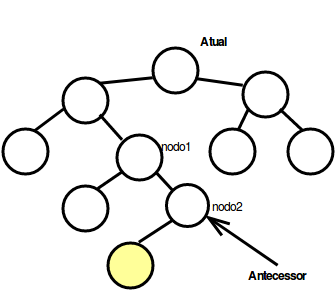
\includegraphics[width=130pt]{imagens/remover_atual1.png}
  \label{fig_remover_atual1}
\end{figure}
\end{frame}

%------------------------------------------------

\begin{frame}{Árvore Binária de Busca}{Função RemoverAtual}

\begin{itemize}
\item Ao executar o comando da linha \ref{atualiza_nodo1_dir}:
\[
  nodo1.dir \leftarrow nodo2.esq,
\]
nodo1 herda o filho da esquerda de nodo2, conforme a figura abaixo.
\end{itemize}

\begin{figure}[!h]
  \centering
  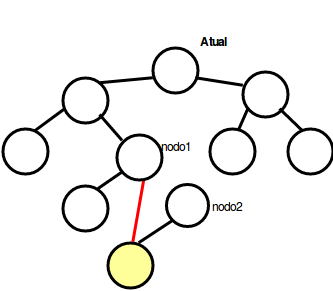
\includegraphics[width=130pt]{imagens/remover_atual2.png}
  \label{fig_remover_atual2}
\end{figure}
\end{frame}

%------------------------------------------------

\begin{frame}{Árvore Binária de Busca}{Função RemoverAtual}
\begin{itemize}
\item O próximo comando, linha \ref{atualiza_nodo1_esq}:
\[
  nodo2.esq \leftarrow atual.esq
\]
faz com que nodo2 herde o filho da \underline{esquerda} do nodo a ser removido, o nodo raiz, conforme a figura abaixo.
\begin{figure}[!h]
  \centering
  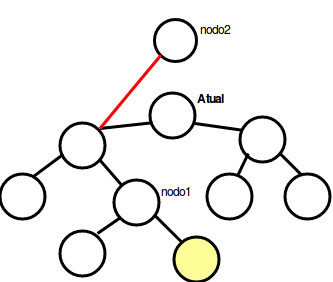
\includegraphics[width=130pt]{imagens/remover_atual3.png}
  \label{fig_remover_atual3}
\end{figure}
\end{itemize}
\end{frame}

%------------------------------------------------

\begin{frame}{Árvore Binária de Busca}{Função RemoverAtual}
\begin{itemize}
\item O último comando desta etapa, linha \ref{atualiza_filhos_fim}:
\[
  nodo2.dir \leftarrow atual.dir
\]
faz com que nodo2 herde o filho da \underline{direita} do nodo a ser removido, o nodo raiz, conforme a figura abaixo.
\begin{figure}[!h]
  \centering
  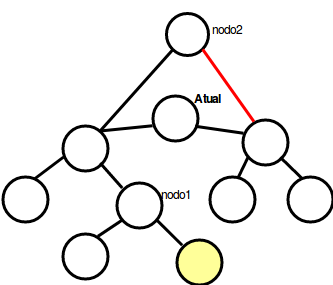
\includegraphics[width=130pt]{imagens/remover_atual4.png}
  \label{fig_remover_atual4}
\end{figure}
\end{itemize}
\end{frame}


\begin{frame}{Árvore Binária de Busca}{Função RemoverAtual}
\begin{itemize}
\item Observe que as linhas \ref{atualiza_nodo1_dir} e \ref{atualiza_nodo1_esq} não são executadas caso o pai do nodo antecessor seja igual ao nodo {\bf atual}, ou seja executa apenas se {\bf (nodo1 $\neq$ atual)}, pois se (nodo1 = atual) a subárvore da esquerda não será alterada.
\item Isso ocorre, quando tem-se a situação mostrada na figura abaixo.
\begin{figure}[!h]
  \centering
  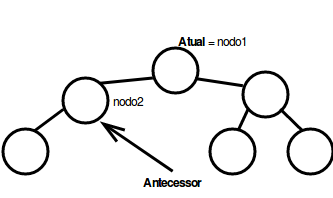
\includegraphics[width=130pt]{imagens/remover_atual5.png}
  \label{fig_remover_atual5}
\end{figure}
\item O comando da linha  \ref{atualiza_filhos_fim} é executado independente de $nodo1 \neq atual$ ( o nodo antecessor ser o filho da esquerda do nodo atual).
\end{itemize}
\end{frame}
%------------------------------------------------

\begin{frame}{Árvore Binária de Busca}{Função RemoverAtual}
\begin{itemize}
 \item Ao fim desta etapa, do laço {\bf enquanto}, o {\bf nodo2} aponta para o \underline{antecessor}, e {\bf nodo1} aponta para o \underline{pai do antecessor}.
\end{itemize}
\end{frame}

%------------------------------------------------

\begin{frame}{Árvore Binária de Busca}{Função RemoverÁrvore}
\begin{itemize}
 \item Para remover um elemento, tem-se três casos a serem tratados:
 \begin{enumerate}
 \item Caso o nodo a ser removido seja a raiz.
 \begin{itemize}
 \item Nesse caso, busca seu antecessor e este passa a ser a nova raiz.
 \end{itemize}
 \item Caso contrário, verifica se o nodo a ser removido está à direita de seu pai.
 \begin{itemize}
 \item Busca o antecessor e este passa a ser o filho à direita do pai do nodo a ser removido.
 \end{itemize}
 \item Ou se está à esquerda de seu pai.
 \begin{itemize}
 \item Busca o antecessor e este passa a ser o filho à esquerda do pai do nodo a ser removido.
 \end{itemize} 
 \end{enumerate}
\end{itemize}
\end{frame}

%------------------------------------------------

\begin{frame}{Árvore Binária de Busca}{Função RemoverÁrvore}
\scalebox{0.45}{
\begin{algorithm}[H]
\caption{RemoverArvore} 
\label{RemoverArvore}
\Entrada{Ponteiro $r$ para raiz, item $x$ a ser removido na árvore.}
\Saida{Retorna V ou F.}
\Inicio{
  \Se {(r=NULL)} { \label{remover_arvore_vazio_inicio}
    \Retorna Falso 
  } \label{remover_arvore_vazio_fim}
  anterior $\leftarrow$ NULL \\
  atual $\leftarrow$ r \\
  \Enqto{(atual $\neq$ NULL)} {
    \Se {(valor = atual.item)} { \label{remover_arvore_inicio}
      	\Se{(atual = r)} {
			r $\leftarrow$ RemoveAtual(atual)\\
      	}
     	\Senao {
			\Se {(anterior.dir = atual)} {
	  			anterior.dir $\leftarrow$ RemoverAtual(atual)\\
			}
			\Senao {
	  			anterior.esq $\leftarrow$ RemoverAtual(atual)\\
			}	
      	}
      	\Retorna Verdadeiro
    }  \label{remover_arvore_fim}
    \Senao { \label{remover_arvore_caminho_inicio}
      	anterior $\leftarrow$ atual\\
      	\Se{(x $>$ atual.item)} {
			atual $\leftarrow$ atual.dir \\
      	}
      	\Senao {
			atual $\leftarrow$ atual.esq \\
      	}
    }\label{remover_arvore_caminho_fim}
  }
  \Retorna Falso
}
\end{algorithm}
}  

\tiny{Adaptado de \cite{Backes2016}}
\end{frame}


%------------------------------------------------

\begin{frame}{Árvore Binária de Busca}{Função RemoverÁrvore}
\begin{itemize}
 \item Primeiramente, verifica se a raiz $r$ é igual a NULL (linha \ref{remover_arvore_vazio_inicio} ).
 \begin{itemize}
 \item Caso seja verdadeiro, retorna falso indicando um erro: a árvore está vazia (linha \ref{remover_arvore_vazio_fim}).
 \end{itemize}
 \item Para buscar o elemento a ser removido, cria-se dois ponteiros auxiliares:
 \begin{itemize}
 \item {\bf atual}, ponteiro utilizado para caminhar na árvore. 
 \item {\bf anterior}, pai do ponteiro {\bf atual} .
 \end{itemize}  
 \item O laço de repetição {\bf enquanto} termina quando {\bf atual} é igual a NULL, o que indica que o elemento a ser removido não foi encontrado.
\end{itemize}
\end{frame}


%------------------------------------------------

\begin{frame}{Árvore Binária de Busca}{Função RemoverÁrvore}
\begin{itemize}
 \item Dentro do laço de repetição, tem-se duas operações:
 \begin{enumerate}
 \item Caso encontre o nodo, o remove (linha \ref{remover_arvore_inicio} até \ref{remover_arvore_fim}).
 \item Caso não encontre, caminha na árvore a fim de encontrá-lo (linha \ref{remover_arvore_caminho_inicio} até \ref{remover_arvore_caminho_fim}).
 \end{enumerate}
 \item Ao encontrar o nodo a ser removido, tem-se três situações:
 \begin{enumerate}
  	\item Caso o nodo a ser removido seja a raiz ({\bf atual = $r$}).
    \begin{itemize}
    	\item Chama a função RemoveAtual, o nodo antecessor de $r$ passa a ser a nova raiz.
    \end{itemize}
  	\item Caso não seja a raiz, verifica se o nodo a ser removido está à direita de seu pai.
  	\begin{itemize}
  	\item Chama a função RemoveAtual, que retorna o substituto do nodo {\bf atual}, e este passa a ser o filho à direita do pai do nodo a ser removido.
  	\end{itemize}
  	\item Caso contrário, o nodo a ser removido está à esquerda de seu pai.
  	\begin{itemize}
  	\item Idêntico ao anterior, no entanto o substituto passa a ser o filho à esquerda do pai do nodo a ser removido.
  	\end{itemize}  	
 \end{enumerate} 
\end{itemize}
\end{frame}


%------------------------------------------------

\begin{frame}{Árvore Binária}{Implementação}
\begin{itemize}
\item Para apagar uma árvore, deve-se:
 \begin{itemize}
 \item Apagar recursivamente suas subárvores
 \item Em seguida, apagar o nodo raiz.
 \end{itemize} 
 \item As chamadas recursivas param ao encontrar uma subárvore vazia, ou seja, quando ({\bf r == NULL})
 \end{itemize} 
\end{frame}

%------------------------------------------------

\begin{frame}{Árvore Binária de Busca}{Apaga Árvore}
% \scalebox{0.8}{
\begin{algorithm}[H]
\caption{ApagarÁrvore} 
\label{ApagarArvore}
\Entrada{Ponteiro $r$ para raiz da árvore a ser apagada.}
\Inicio{
  \Se{(NOT(ÁrvoreVazia(r)))} {
    ApagarÁrvore(r.esq) \\ 
    ApagarÁrvore(r.dir) \\
    DESALOCA\_NODO(r) \\
  }
}
\end{algorithm}
% }
\tiny{Adaptado de \cite{Backes2016}}  
\end{frame}


% -----------------------------------

\section{Conclusão}

\begin{frame}{Conclusão}
\begin{itemize}
  \item No pior caso, pode acontecer da árvore ficar {\bf degenerada}.
  \begin{itemize}
  \item Cada nodo possui um único filho.
  \item Sua estrutura é igual a uma lista linear.
  \item A altura $h$ da árvore será: $h = n -1$
\end{itemize}
  \item Isso dependerá da ordem em que os elementos são inseridos na árvore.
  \item Caso isso ocorra, o custo das operações é linear ($O(n)$).
  \item A fim de evitar seu degeneramento, pode-se realizar o seu balanceamento. 
  \item A seguir, um exemplo de árvore degenerada.
\begin{figure}[!h]
  \centering
  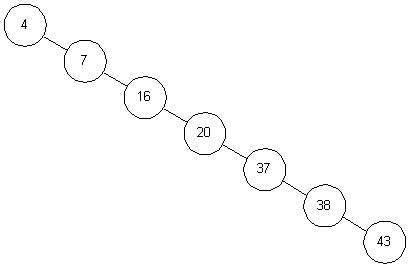
\includegraphics[width=150pt]{imagens/arvore_degenerada.png}
  \label{fig_arvore_degenerada}
\end{figure}
 \end{itemize}
\end{frame}

% -----------------------------------

\begin{frame}{Referências}{Bibliografia Básica}

\begin{itemize}
\item Bibliografia Básica
\bibliographystyle{abnt-alf}
\bibliography{referencias}
\item Material Complementar
\begin{itemize}
\item \href{https://programacaodescomplicada.wordpress.com/complementar/}{Link código-fonte e listas de exercícios- Material disponível on-line}
\end{itemize}
\item Animação
\begin{itemize}
\item \href{https://www.cs.usfca.edu/~galles/visualization/BST.html}{Link Árvore Binária de Busca}
\item \href{http://btv.melezinek.cz/binary-search-tree.html}{Link Árvore Binária de Busca - Versão que utiliza sucessor como nodo subtituto na remoção.}
\end{itemize}
\end{itemize}
\end{frame}

%------------------------------------------------
\begin{frame}
\titlepage % Print the title page as the first slide

\begin{figure}[!h]
  \centering
   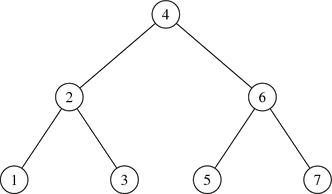
\includegraphics[width=120pt]{imagens/introducao.png}
  \label{fig_introducao}
\end{figure}
\end{frame}

%----------------------------------------------------------------------------------------


\end{document} 
